\documentclass[a4paper,12pt]{article}

% Configuração de idioma e codificação
\usepackage[utf8]{inputenc}
\usepackage[T1]{fontenc}
\usepackage[brazil]{babel}

% Layout da página
\usepackage[a4paper, margin=0.8in]{geometry}
\usepackage{setspace}
\setstretch{1.5} % Espaçamento entre linhas

\usepackage{amsmath, bm} % Pacotes matemáticos
\usepackage{graphicx} % Inclusão de imagens
\usepackage{caption} % Estilização de legendas
\usepackage{fancyhdr} % Personalização de cabeçalhos e rodapés
\usepackage{titlesec} % Personalização de títulos de seção
\usepackage{xcolor} % Cores para textos e seções
\usepackage{hyperref} % Links clicáveis
\usepackage{background} % Fundo para a página de título
\usepackage{placeins} % Controle de posicionamento de floats (FloatBarrier)
\usepackage{pdfpages}
\usepackage{enumitem}
% Ensure the package is loaded correctly for \floatbarrier

\hypersetup{
    colorlinks=true,
    linkcolor=red,
    urlcolor=red,
    citecolor=red
}

% Personalização dos títulos
\titleformat{\section}{\Large\bfseries\color{black}}{\thesection}{1em}{}
\titleformat{\subsection}{\large\bfseries\color{black}}{\thesubsection}{1em}{}

% Cabeçalhos e Rodapés
\pagestyle{fancy}
\fancyhf{}
\fancyhead[R]{
\includegraphics[width=2cm]{ITA.png}} % Logo no topo direito
\fancyhead[L]{\textbf{Instituto Tecnológico de Aeronáutica (ITA)}}
\fancyfoot[L]{Leonardo Peres Dias}
\fancyfoot[R]{\thepage}

% Informações do título
\title{
    \textbf{Inteligência Artificial para Robótica Móvel CT-213}\\
    \Large Instituto Tecnológico de Aeronáutica 

    \textbf{Relatório do Laboratório 11 -  Aprendizado por Reforço Livre de Modelo}\\
}
\author{
    Leonardo Peres Dias 
}
\date{\today}

% Configuração do fundo (marca d'água apenas na primeira página)
\backgroundsetup{
    scale=1.5,
    color=black,
    opacity=0.2,
    angle=0,
    position=current page.south,
    vshift=5cm,
    hshift=0cm,
    contents={
\includegraphics[width=8cm]{ITA.png}}
}

% Início do Documento
\begin{document}

% Aplicar o fundo apenas na primeira página
\BgThispage
\maketitle
\thispagestyle{empty} % Sem cabeçalho/rodapé na página de título

%\begin{abstract}
%Este documento apresenta o relatório do Projeto CES-30 - 2024, desenvolvido com base na segunda forma descrita no enunciado do exame. O projeto abrange tarefas de \textbf{mineração de dados} e \textbf{construção de grafos de conhecimento}, com a aplicação de técnicas específicas para análise e solução prática de problemas reais.
%\end{abstract}

\newpage
\NoBgThispage % Desativa a marca d'água para as páginas seguintes

\tableofcontents

\newpage
\NoBgThispage % Desativa a marca d'água para as páginas seguintes

\section{Breve Explicação em Alto Nível da Implementação}
A implementação desenvolvida define uma classe base \texttt{RLAlgorithm}, e suas especializações \texttt{Sarsa} e \texttt{QLearning}.

A tabela de ação-valor (\textit{Q-table}) é representada por uma matriz \texttt{q} de dimensão \texttt{(num\_states, num\_actions)}. Cada entrada \texttt{q[s, a]} corresponde à execução da ação $a$ no estado $s$ sob a política corrente.

\subsection{SARSA}

O algoritmo SARSA segue uma política \textit{on-policy}, ou seja, utiliza a mesma política $\varepsilon$-greedy tanto para seleção de ações quanto para atualização dos valores. A função \texttt{learn} atualiza a Q-table de acordo com a seguinte equação:

\[
Q(s, a) \leftarrow Q(s, a) + \alpha \left[ r + \gamma Q(s', a') - Q(s, a) \right]
\]

onde $a'$ é a próxima ação escolhida de acordo com a política $\varepsilon$-greedy.

\subsection{Q-Learning}

Já o Q-Learning é um algoritmo \textit{off-policy}, ou seja, aprende assumindo que sempre será tomada a melhor ação futura, mesmo que a execução atual use uma política $\varepsilon$-greedy. A atualização da Q-table segue a equação:

\[
Q(s, a) \leftarrow Q(s, a) + \alpha \left[ r + \gamma \max_{a'} Q(s', a') - Q(s, a) \right]
\]

Ambos os algoritmos utilizam funções auxiliares para seleção de ações (\texttt{epsilon\_greedy\_action}, \texttt{greedy\_action}) e para gerar a política determinística greedy em forma tabular a partir da Q-table final (\texttt{compute\_greedy\_policy\_as\_table}).

\newpage
\section{Figuras Comprovando Funcionamento do Código}

\subsection{SARSA}
\begin{enumerate}[label=2.1.\arabic*.]
    \item \textbf{Tabela Ação-Valor e Política \textit{Greedy} Aprendida no Teste com MDP Simples}\\
    
    \begin{table}[h!]
    \centering
    \caption{Tabela Ação-Valor Q(s,a) aprendida pelo SARSA}
    \begin{tabular}{|c|c|c|c|}
    \hline
    \textbf{Estado $s$} & \textbf{Q(s, Ação = L)} & \textbf{Q(s, Ação = S)} & \textbf{Q(s, Ação = R)} \\
    \hline
    0 & -9.33 & -8.60 & -10.58 \\
    1 & -10.47 & -9.64 & -11.55 \\
    2 & -11.21 & -10.50 & -11.66 \\
    3 & -11.82 & -11.56 & -12.08 \\
    4 & -12.38 & -12.32 & -12.31 \\
    5 & -11.88 & -11.94 & -11.44 \\
    6 & -10.89 & -11.59 & -10.48 \\
    7 & -10.58 & -11.47 & -9.42 \\
    8 & -9.46 & -10.33 & -8.65 \\
    9 & -7.64 & -8.71 & -8.57 \\
    \hline
    \end{tabular}
    \end{table}

    \vspace{0.3cm}

    \noindent\textbf{Política Greedy Aprendida:}


    \[
    \pi = [\text{L}, \text{L}, \text{L}, \text{L}, \text{R}, \text{R}, \text{R}, \text{R}, \text{R}, \text{S}]
    \]
    
    \item \textbf{Convergência do Retorno}\\
    
    \begin{figure}[!h]
    \centering
    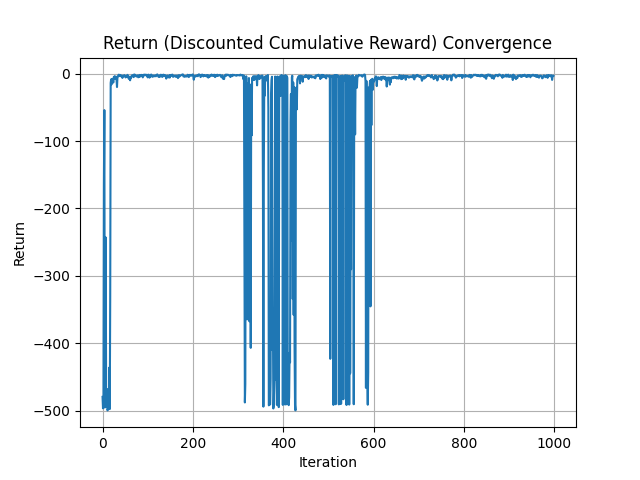
\includegraphics[width=0.6\textwidth]{sarsa/return_convergence.png}
    \caption{Convergência do Retorno no SARSA}
    \label{fig:sarsa_return_convergence}
    \end{figure}
    
    \item \textbf{Tabela Q e Política Determinística que Seria Obtida Através de \textit{Greedy}(Q)}\\
    \begin{figure}[h!]
      \centering
      \begin{minipage}{0.5\textwidth}
        \centering
        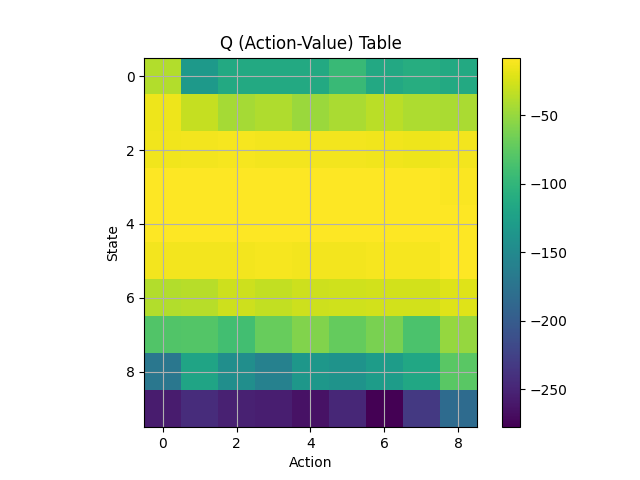
\includegraphics[width=\textwidth]{sarsa/action_value_table.png}
        \caption{Tabela Q aprendida pelo SARSA}
        \label{fig:sarsa_q_table}
      \end{minipage}\hfill
      \begin{minipage}{0.5\textwidth}
        \centering
        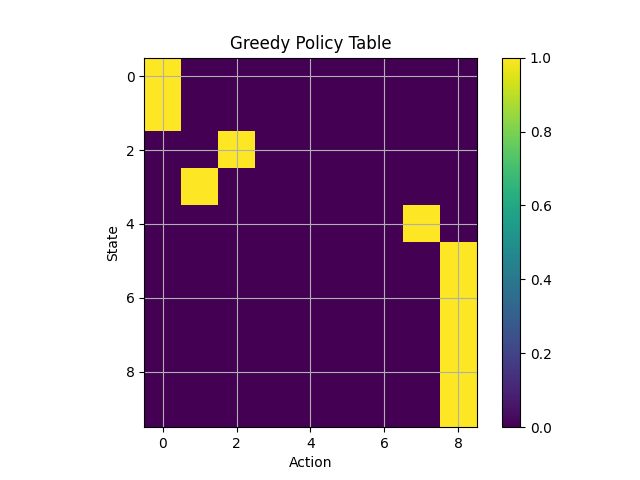
\includegraphics[width=\textwidth]{sarsa/greedy_policy_table.png}
        \caption{Política determinística Greedy obtida}
        \label{fig:sarsa_greedy_policy}
      \end{minipage}
    \end{figure}
    
    \item \textbf{Melhor Trajetória Obtida Durante o Aprendizado}\\
    \begin{figure}[!h]
    \centering
    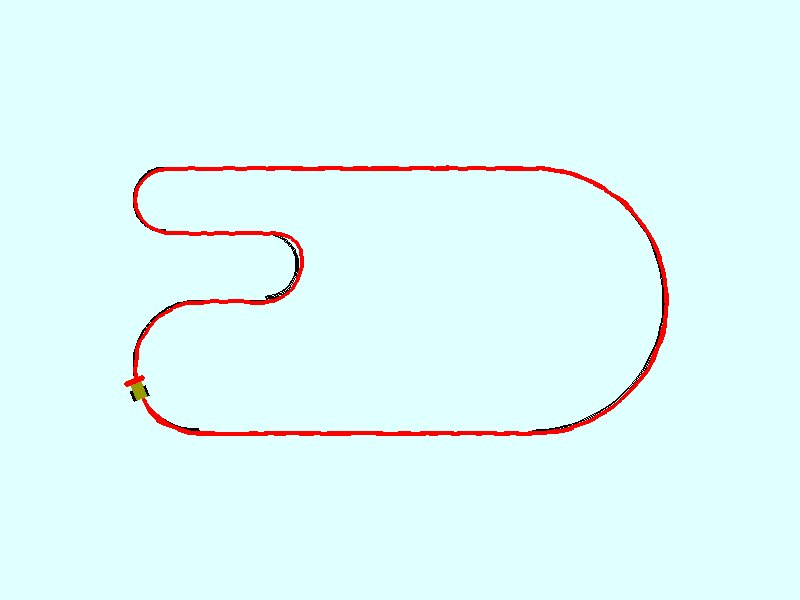
\includegraphics[width=0.6\textwidth]{sarsa/line_follower_solution.jpeg}
    \caption{Melhor Trajetória Obtida pelo SARSA}
    \label{fig:sarsa_best_trajectory}
    \end{figure}
\end{enumerate}

\newpage
\subsection{Q-Learning}
\begin{enumerate}[label=2.2.\arabic*.]
    \item \textbf{Tabela Ação-Valor e Política \textit{Greedy} Aprendida no Teste com MDP Simples}\\
    
    \begin{table}[h!]
    \centering
    \caption{Tabela Ação-Valor Q(s,a) aprendida pelo Q-Learning}
    \begin{tabular}{|c|c|c|c|}
    \hline
    \textbf{Estado $s$} & \textbf{Q(s, Ação = L)} & \textbf{Q(s, Ação = S)} & \textbf{Q(s, Ação = R)} \\
    \hline
    0 & -1.99 & -1.00 & -2.97 \\
    1 & -2.97 & -1.99 & -3.94 \\
    2 & -3.45 & -2.97 & -4.55 \\
    3 & -4.14 & -3.94 & -4.49 \\
    4 & -5.19 & -4.89 & -4.89 \\
    5 & -4.25 & -4.60 & -3.94 \\
    6 & -3.75 & -4.11 & -2.97 \\
    7 & -2.97 & -3.91 & -1.99 \\
    8 & -1.99 & -2.97 & -1.00 \\
    9 &  0.00 & -0.99 & -0.99 \\
    \hline
    \end{tabular}
    \end{table}

    \vspace{0.3cm}

    \noindent\textbf{Política Greedy Aprendida:}

    \[
    \pi = [\text{L}, \text{L}, \text{L}, \text{L}, \text{L}, \text{R}, \text{R}, \text{R}, \text{R}, \text{S}]
    \]
    
    \item \textbf{Convergência do Retorno}\\
    \begin{figure}[!h]
    \centering
    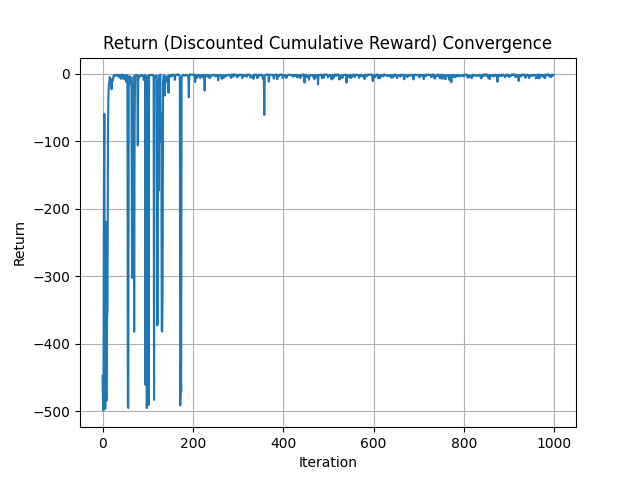
\includegraphics[width=0.6\textwidth]{q-learning/return_convergence.png}
    \caption{Convergência do Retorno no Q-Learning}

    \end{figure}

    \newpage
    
    \item \textbf{Tabela Q e Política Determinística que Seria Obtida Através de \textit{Greedy}(Q)}\\
    \begin{figure}[h!]
      \centering
      \begin{minipage}{0.5\textwidth}
        \centering
        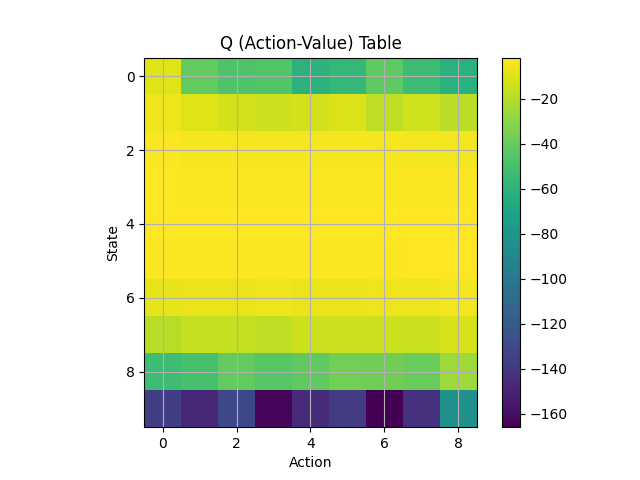
\includegraphics[width=\textwidth]{q-learning/action_value_table.png}
        \caption{Tabela Q aprendida pelo Q-Learning}

      \end{minipage}\hfill
      \begin{minipage}{0.5\textwidth}
        \centering
        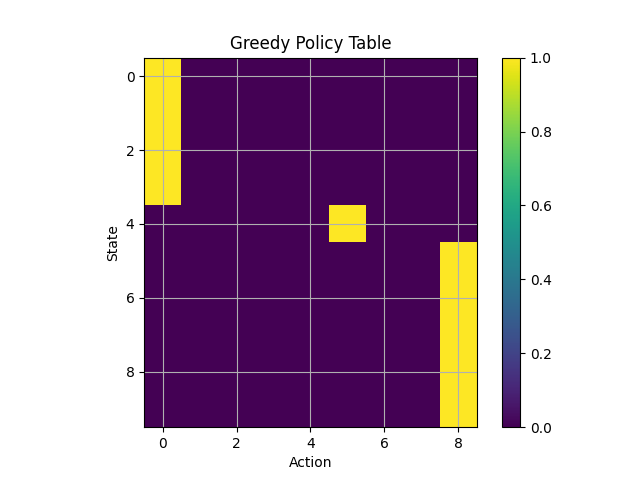
\includegraphics[width=\textwidth]{q-learning/greedy_policy_table.png}
        \caption{Política determinística Greedy obtida}

      \end{minipage}
    \end{figure}
    
    \item \textbf{Melhor Trajetória Obtida Durante o Aprendizado}\\
    \begin{figure}[!h]
    \centering
    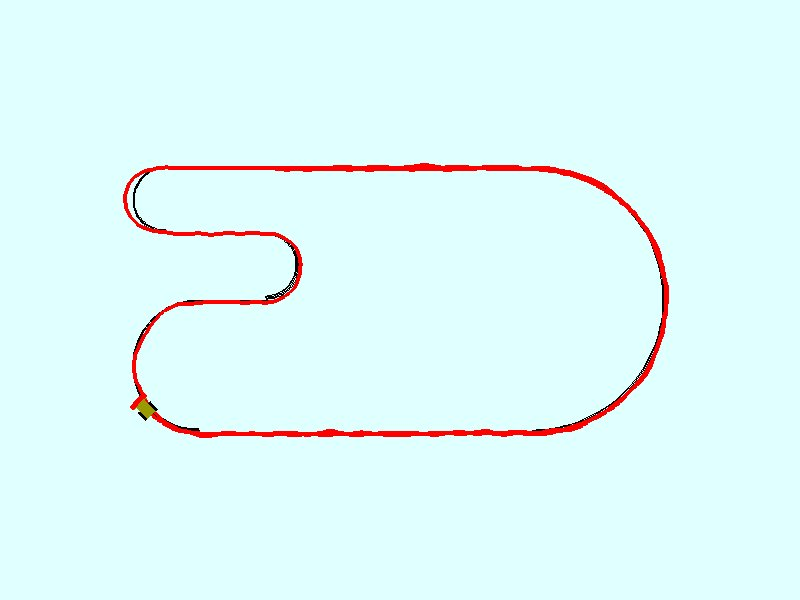
\includegraphics[width=0.6\textwidth]{q-learning/line_follower_solution.jpeg}
    \caption{Melhor Trajetória Obtida pelo Q-Learning}
    \end{figure}
\end{enumerate}


\newpage
\section{Discussão dos Resultados}

No experimento com o MDP simplificado — um labirinto unidimensional — tanto o algoritmo SARSA quanto o Q-Learning convergiram para políticas \textit{greedy} que resolvem a tarefa de forma ótima. Ambas as políticas levam o agente da posição inicial até o objetivo com o menor número possível de passos. No entanto, apesar de serem ótimas, as políticas aprendidas diferem: por exemplo, no estado central do labirinto, a ação ótima aprendida pelo SARSA foi virar à direita, enquanto o Q-Learning optou por virar à esquerda — ambas válidas devido à simetria do ambiente. Essa diferença reflete o caráter \textit{on-policy} do SARSA, que tende a aprender com base no comportamento atual, e o aspecto \textit{off-policy} do Q-Learning, que favorece estimativas mais agressivas das melhores ações. Além disso, os valores nas tabelas de ação-valor mostram que o Q-Learning atribui valores mais altos (menos negativos), indicando uma política mais otimista em relação ao retorno esperado.

Nos testes realizados com o robô seguidor de linha, observamos que ambos os algoritmos — SARSA e Q-Learning — foram capazes de aprender trajetórias que completam o percurso de forma eficaz. Contudo, a convergência do retorno apresentou comportamentos distintos: o SARSA exibiu maior instabilidade ao longo das iterações, com episódios de retorno significativamente negativos, especialmente nas fases iniciais do aprendizado. Isso reflete seu caráter \textit{on-policy}, que o torna mais sensível à política exploratória. Por outro lado, o Q-Learning convergiu de forma mais estável e rápida, beneficiando-se de seu viés \textit{off-policy} e natureza mais otimista. As tabelas de ação-valor ilustram essa diferença, com valores mais consistentes e homogêneos para o Q-Learning. No geral, apesar de trajetórias semelhantes terem sido obtidas ao final do treinamento, o Q-Learning demonstrou maior robustez e confiabilidade durante o processo de aprendizado.
% (Escreva aqui uma análise crítica comparando os resultados de SARSA e Q-Learning)
\end{document}